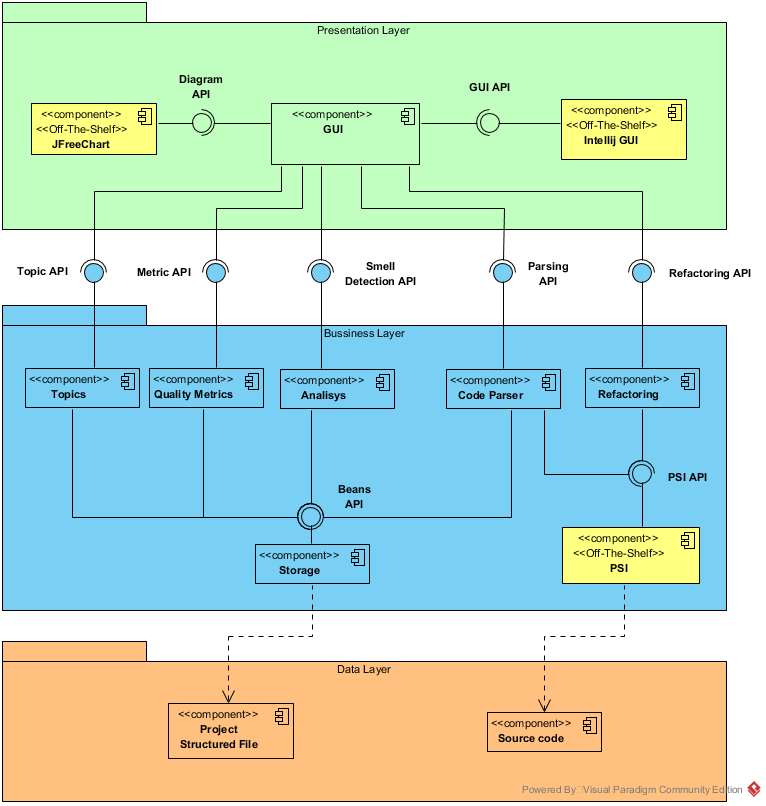
\includegraphics[scale=0.85]{PS_Architecture/diagrams_PNG/Component_Diagram.png}\\
\centering
\textbf{Component Diagram}\\

\flushleft

\begin{tabular}{|l|p{13cm}|}
	\hline
	\textbf{\Large Name} & \textbf{\Large Descrizione} \rule[-1cm]{0mm}{2cm} \\ \hline
	
	\textbf{Analisi} &  Componente che si occupa di analizzare il codice java identificando, tramite metriche e topic ottenute da altre componenti, la presenza di code smell.
	\rule[-1cm]{0mm}{1cm} \\ \hline
	\textbf{Refactoring} & Componente che si occupa di generare una possibile soluzione ad un code smell selezionato presente all'interno del codice java in analisi, procedendo poi all'eventuale applicazione di quest'ultima risolvendo così il code smell identificato. 
	\rule[-1cm]{0mm}{1cm} \\ \hline
	\textbf{Storage} & Componente gestisce l'accesso al file strutturato del progetto in analisi
	\rule[-1cm]{0mm}{1cm} \\ \hline
	\textbf{GUI} & Componente che realizza l'interfaccia grafica, la quale si appoggia su Intellij API(per componenti grafiche) e JFreeChart(per grafici). 
	\rule[-1cm]{0mm}{1cm} \\ \hline
	\textbf{Code Parser} & Componente che prende la struttura elaborata dal PSI come input ed, estrapolando informazioni da questo, costruisce i Beans fornendo così una diversa rappresentazione strutturata dell'input.
	\rule[-1cm]{0mm}{1cm} \\ \hline
	\textbf{Quality Metrics} & Componente che si occupa del calcolo delle metriche qualitative quali LOC, WNC, RFC, CBO, LCOM, NOA, NOM, NOPA e NOP.
	\rule[-1cm]{0mm}{1cm} \\ \hline
	\textbf{Topics} & Componente che si occupa del calcolo dei topic ovvero dei termini più ricorrenti all'interno del codice analizzato.
	\rule[-1cm]{0mm}{1cm} \\ \hline	
	\textbf{Project Structured File} & Componente che implementa una meccanica di cache realizzata in SQLite come singolo DB di cache per ogni progetto (descritta nel dettaglio nella sezione del Persistent data management).
	\rule[-1cm]{0mm}{1cm} \\ \hline	
\end{tabular}

